

The system is designed as two complementary components:

\begin{enumerate}
    \item A corpus profiling tool, which produces a metadata-only description of the corpus as a multivariate distribution;
    \item A targeted retrieval tool, that attempts to produce a corpus with the same distribution.
\end{enumerate}



\section{Profiling}
The process of constructing a corpus description may be started either from a seed corpus, or from direct user design.

\begin{figure}[h]
    \centering
    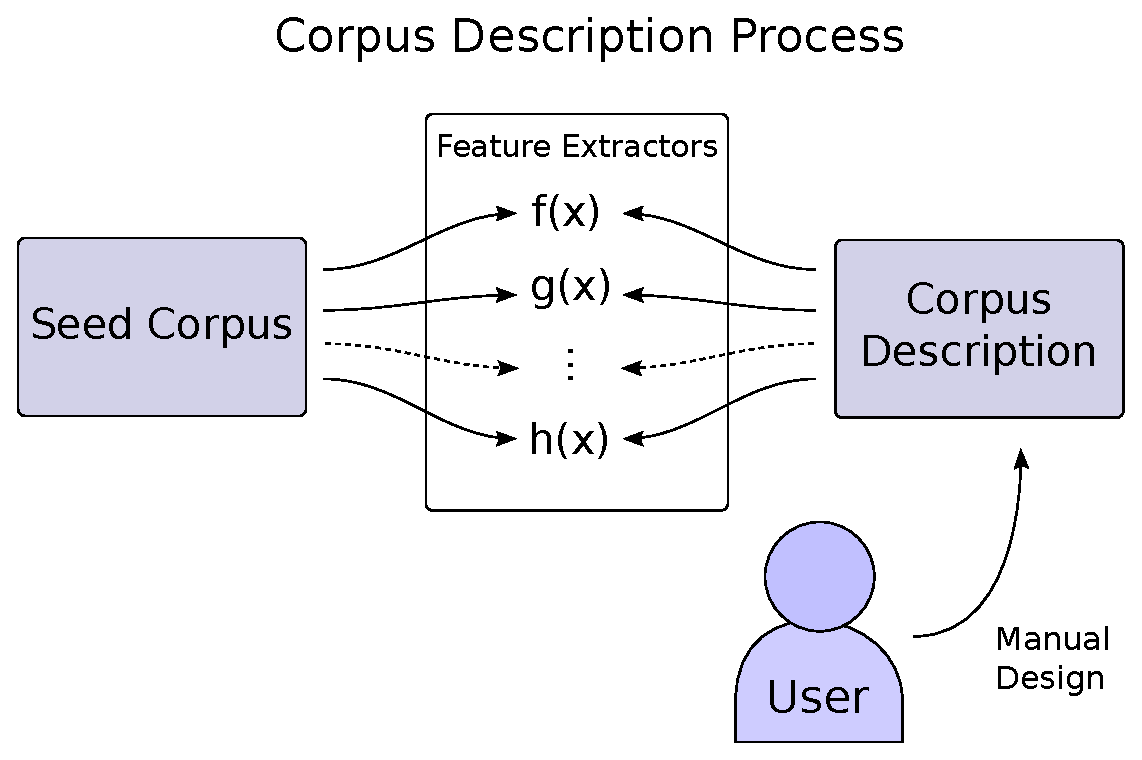
\includegraphics[width=0.8\textwidth]{rebuilding/profiling}
    \caption{Creation of a corpus description}
    \label{fig:rebuilding:profiling}
\end{figure}


The process of building a corpus description is outlined in~\ref{fig:rebuilding:profiling}.  For direct use, the user would specify their salient dimensions, and the distribution for each.  This is essentially a description of the sampling policy---where variables are discrete and nominal (such as genre labels), this would take the form of a table with desired proportions against each.  Where variables are continuous, a probability density function is defined.  Note that this method does not, without prohibitive complexity, allow for specification of interactions between variables\td{return to this and comment on it later}.

Profiling through the use of a `seed' corpus begins with specifications of the salient dimensions, the data for which are then read from the seed (by $f()$ and $g()$ functions in the figure).  As each document is read, the corpus description may contain information not only on marginal distributions for each variable, but also the effects of conditioning on one or more value.

Note that, whichever method is used, this stage is merely a metadata description task.  The corpus description document itself contains no more information than the metadata of the corpora from which is it built---indeed, where all variables are both external and nominal, this reduces to a simple table of frequencies for each desired value.  

Those specifying variables to describe must, as with all sampling, be mindful of their potential systematic correlations with variables of interest to any given research question.  The value of this approach is in documentation---it is possible for a researcher to eyeball the variables (and potentially their distributions) and determine whether or not a corpus is correctly conditioned for use inferring about a given variable.  This cannot be said for bootstrapping systems that use internal variables, which seek to copy corpus contents at the risk of varying their metadata.


% ---

\section{Retrieval}
Retrieval in accordance with the complex distributions specified in a corpus description is challenging in two ways:

\begin{itemize}
    \item Samples must be taken from the corpus description in accordance with a complex empirically-determined distribution;
    \item Any combination of variables sampled from the distribution must then be sought based on its metadata alone.
\end{itemize}

The former of these is difficult because many seed corpora may lack sufficient data to specify their distributions, and because of the high dimensionality of the distributions in question.  These issues may be addressed using techniques such as Gibbs, slice, or rejection sampling.  



\subsection{Resampling}

\td{cite this}
\begin{figure}[h]
    \centering
    \includegraphics[width=0.8\textwidth]{rebuilding/resampling}
    \caption{Resampling the corpus using MCMC methods}
    \label{fig:rebuilding:resampling}
\end{figure}



Resampling from the original corpus produces a `prototype' document, which has values of metadata fields that, over time, hold the same distribution as those in the seed corpus.  To perform this resampling, we must be able to sample from a distribution proportional to that of each variable conditional on all of the others, requiring that the corpus description contains information on interactions between values.

The process of constructing a new corpus is one of continually producing these `prototypes' conditional on the values of metadata already sampled, and then retrieving the text for each.  Resampling according to multivariate distributions is possible using Gibbs or slice sampling, both of which are MCMC techniques---the `output' distribution of prototype metadata will iteratively approach the distribution of input data.

This process is nonparametric, and thus able to accept arbitrary empirical input distributions and arbitrary modifications thereto.  This allows us to arbitrarily boost the sampling probability of a given category, or to ensure that variables with hitherto-unseen values are considered contributory to the output corpus.

Gibbs sampling is also commonly used to infer the posterior distribution of individual variables by fixing the values of the input distributions.  Though beyond the scope of this thesis, it would be possible to use this technique to fix input variables and identify the distribution of metadata values also described in the corpus description document.  This technique would be highly sensitive to the bias of the retrieval mechanism, and would require a particularly large seed corpus to operate meaningfully.


\til{
Theoretically speaking, the corpus is reconstructed as a distribution of all internal variables on the document, conditional on the values in the metadata.  So long as the retrieval engine can find documents fitting the distribution of input data, the output data will conform to the posterior distribution of word frequencies (or any other internal property one wishes to reason about).

Separation of the latent (internal) variables into a block is consistent with a 'block gibbs sampler'.  Ignoring them as a block is consistent with a 'collapsed gibbs sampler'.

% This is awesome: http://www.people.fas.harvard.edu/~plam/teaching/methods/mcmc/mcmc_print.pdf
}


\til{ Describe gibbs formally, and compare slice to it.  Describe the process of resampling from the output using the input distribution. }









